\documentclass{ctuthesis}
\usepackage{mathtools}
\ctusetup{
xdoctype = B,
xfaculty = F3,
mainlanguage = english,
secondlanguage = czech,
title-english = {Planning routes for recreational cycling},
title-czech = {Plánování tras pro rekreační cyklistiku},
department-english = {Department of Computer Science},
author = {Miroslav Matocha},
supervisor = {doc. Ing. Michal Jakob, Ph.D.},
supervisor-address = {Fakulta elektrotechnická, Resslova 307/9, Praha},
month = 6,
year = 2019,
day = 6,
keywords-english = {route planning, cycles},
keywords-czech = {plánování cest, cykly}
}

\ctuprocess
\begin{abstract-english}
This paper is focused on problem of planning enclosed circular walks in graph constrained by length and optimizing criterion of pleassantnes. It examines various work in this field. Then from this work is chosen one state of the the art algorithm, which is described in more specific theoretical way. Introducing some particular concepts used in solution as is working with walk roundness or geospatial diversity of generated routes. Implementation of chosen algorithm is also part of this work. This implementation is further tested on various instances of problem and its results are further discussed.
\end{abstract-english}
\begin{abstract-czech}
Tato práce je zaměřená na problém nalezení kružnic v grafu, které jsou omezeny délkou a přitom optimalizují kritérium příjemnosti. Zkoumá rozličné postupy v této oblasti. Poté je vybrán specifický algoritmus, který je teoreticky rozebrán ve větším detailu. Během toho práce rozebírá několik specifických konceptů použitých při řešení problému, jako je třeba práce s kulatostí vybrané kružnice, nebo geografická diversita mezi nalezenými řešeními. Součástí této práce je také implementacevybraného algoritmu. Tato implementace je dále testována na rozličných instancích problému a její výsledky jsou diskutovány.
\end{abstract-czech}


% Acknowledgements / Podekovani
\begin{thanks}
Thanks to CTU for beeing so great \emph{alma mater}.
\end{thanks}

% Declaration / Prohlaseni
\begin{declaration}
I declare that I wrote this paper by myself and that I mentioned all used literature in bibliography section.

In Prague, \ctufield{day}.~\monthinlanguage{title}~\ctufield{year}
\end{declaration}


\begin{document}
\maketitle
\chapter{Introduction}
People are nowadays pretty used to planning and navigating their trips with the help of various map applications, thank to the rapid spread of GPS technology especially in mobile phones in the past years. The problem of getting from A to B by the best route possible is, thanks to this intensive usage and various achievments in this field, practically completely solved. These are also the reason why people are starting to get into other areas of planning trips and trying to apply obtained knowledge to wider set of problems. This for example includes multicriterial planning or planning in dynamic networks. \par
In this paper I am focused to break down the problem of using algorithmically planned routes for recreational activities, which is specific for several reasons. For example people which are interested in using generated routes for jogging or cycling are just rarely interested in specific route in terms of visited points or area, they prefer to get several suggestions based on total cost of route instead (in terms of total length or travel time). Actually the most common use case is to plan these routes to form cycles containing the starting point. This is also the use case which I am focused on the most in this paper. Another property of these routes should be optimization of total or mean plesantness. This is whole another aspect of the problem as pleasantness of the edge can mean anything from type of communication through interesting surroundings of the edge to the proximity to some points of interest. It can even mix several criterions and can be personalized to specific user. \par
In the next chapters I will try to  analyze the work which was done in this field in the past, take apart the individual parts of the problem in attempt to formalize it properlly and finally introduce the solution and its implementation which I have created.
\chapter{Related work}


One of the most general papers laying down the theory needed for solution of this problem is problem of finding the minimum mean cycle in the graph. \cite{karp} This problem is defined as finding the circle in the graph which sum of weights through all edges divided by count of edges is minimal. The Karp provides formula which yields the minimum mean of the mentioned cycle with linear complexity. Moreover it shows a simple technique to obtain not only this number but also the actual cycle from the same calculation. \par
The next paper from Gemsa \cite{jogging} introduces several techniques to generate feasible enclosed jogging routes. First it focuses on solving the problem through dual graph which consists of faces from original graph as nodes connected by edges only if the coresponding edges share one of the edges in original graph. This of course requires simple preprocessing step based on right hand deep searches in original graph. After the dual graph is obtained the BFS is run over it starting from node which corresponds to the face incident with starting node. The result of BFS is enclosed jogging route in every iteration. This jogging route is constructed from the border edges of the search tree. This holds as far as two conditions are met. To get simple cycle from border edges the search tree has to be connected. And it has to exclude at least one face incident with starting node to ensure that starting node is part of that border. Both of the properties are constantly checked for during algorithm execution. BFS is finnished as soon as the length criterium is fullfilled. Gemsa introduces one more technique to optimize badness of the jogging route. Another metric influencing the execution of the BFS is added to the mix. This metric consists of force field which assigns a vector to every point in the plannar graph. This vector is counted from simple formula using individual face badness normalized by distance to the power of two. This formula is iterated and summed over all faces in the graph. BFS is then edited in manner of expanding the face which center has the biggest force in the direction of extension. They call this solution Greedy Faces.\par
Second approach which is introduced is called Partial Shortest Paths. This approach is working with computing triangles(or rectangles) which fulfill the length criterion and have starting node as one of its vertices. It does so by computing the search tree of acceptable candidates from starting node. This search tree is called ring and it is constrained by third of the length of the route. From these results one via node is selected and its ring is computed with the same parameters. Then we can take the intersection area and pick the third point from there. Last step is to compute shortest paths between all three mentioned nodes, this yields one of feasible cycles. All the results from this proccess are then filtered to provide just the ones with best mean badness. \par
This approach provide a space for further improvements. For example we could limit the ring bound distance to one fourth of the desired cycle length and pick two points instead of one. From these points we can backtrack a little bit (to improve smothness of the resulting path) and run another two ring searches. In the intersection lies points which are on the path which includes nodes originating the search as well as the nodes from which we backtracked. These nodes are the fourth candidate vertices of the rectangle. Now we can compute shortest paths to complete this rectangle. Results are then filtred in the same manner as before. Algorithm can be further improved by implementing bidirectional search to found the fourth point in the rings intersection. This is also great for paralelization of the algorithm. \par

\chapter{Problem}
We introduce some notation in order to define the problem formally. Our problem is based on undirected graph \(G=(V, E)\). Where every node represent intersection of some sort and edges represents roads in between them. Every one of these edges has its nonegative length. Formally we introduce function \(l:E \rightarrow \mathbb{Z^+}\) which represents this length. We than define path or route of edges which is simply a sequence of edges \(P = [e_1, e_2, ..., e_n]\) where holds that \(SN(e_{i+1}) = EN(e_i) \) for all \(i\) in \(\{2, 3, ..., n\}\) where \(SN\) denotes starting node and \(EN\) ending one. The length of this path is counted as \(w(P)=\sum_{i=1}^{n}{l(e_i)}\). Cycle is special type of path, where \(e_1 = e_n\).

\section{Formal description}
Input to our problem is a mentioned graph \(G=(V, E)\). One starting node \(s \in V\) and the desired length of the final cycle \(l_{des} \in \mathbb{R_+}\). It is impractical and almost impossible to aim for single number as desired length. So we will choose a parameter \(\varepsilon\) which will define interval \(L = (l_{des}-\varepsilon, l_{des}+\varepsilon)\). We will search for cycles \(C\) which fullfill \(w(C) \in L\) and \(s \in C\). And which optimizes the tour pleasantness.
	
\section{Tour pleasantness}

\section{Tour roundness}
Another property which we are interested in is the tour roundness. We could just ban revisitng the edges, but this hard constraint could disqualify a whole range of problem solutions. For example every instance where starting point is located in dead-end street has to be treated specially. As well as instances with large neigbourhoods accessible by one edge only. These would be completely invisible to algorithm with implemented hard constraint. Instead we will describe a functional roundness metric which assigns values between 0 and 1 to every edge of the walk, this value can be later added to the minimalizing term of the algorithm.\par
This metric is based on sinusoidal relation between displacement and distance of two point on the circle (as shown in Fig. 3.1). We obtain displacement between edges by computing distance as crown flies between two GPS locations representing their centers. We will mark this distance as \(d_{real}\). Then we will define \(d_{exp}: E^2 \rightarrow \mathbb{R_+}\) which represents the expected displacement of these centers based on distance of shortest path between these two edges. To use the sinusoidal relation to compute the \(d_{exp}\) we would need to know the final length of the tour, which is not known yet and lies somwhere in \(L\). Instead of using one of interval bounds we will approximate 

\begin{figure}
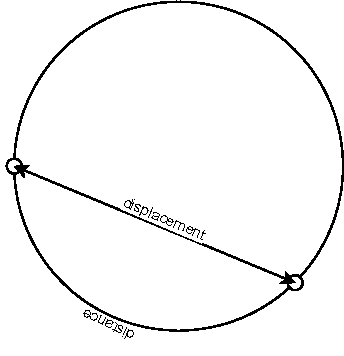
\includegraphics[width=0.4\textwidth]{displacement}
\caption{Ilustration of distance and displacement.}
\end{figure}

\section{Geospatial diversity}

\chapter{Solution proposal}

\chapter{Implementation details}

\section{Implementation description}

\section{Performance results}

\chapter{Conclusion}
Lorep ipsum \cite{stroobant}
\begin{thebibliography}{1}
\bibitem{stroobant}Stroobant, P., Audenaert, P., Colle, D., \& Pickavet, M. (2018). \emph{Generating constrained length personalized bicycle tours.} 4OR, 16(4), 411–439. \url{https://doi.org/10.1007/s10288-018-0371-9} 
\bibitem{karp}Karp, R. M. (1978). \emph{A characterization of the minimum cycle mean in a digraph.} Discrete Mathematics, 23(3), 309–311. \url{https://doi.org/10.1016/0012-365x(78)90011-0} 
\bibitem{oatsp}Maervoet, J., Brackman, P., Verbeeck, K., De Causmaecker, P., \& Vanden Berghe, G. (2013). \emph{Tour Suggestion for Outdoor Activities}. In Web and Wireless Geographical Information Systems (s. 54–63). Springer Berlin Heidelberg. \url{https://doi.org/10.1007/978-3-642-37087-8_5} 
\bibitem{jogging}Gemsa, A., Pajor, T., Wagner, D., \& Zündorf, T. (2013). \emph{Efficient Computation of Jogging Routes.} In Experimental Algorithms (s. 272–283). Springer Berlin Heidelberg. \url{https://doi.org/10.1007/978-3-642-38527-8_25} 
\bibitem{juraska} Juraska, J., Nykl J. (2016). \emph{Multi-criteria Route Planning with Emphasis on Geospatial Result Diversity} \url{https://www.semanticscholar.org/paper/Multi-criteria-Route-Planning-with-Emphasis-on-Juraska-Nykl/96165d905691de3b8e9b0af8b83fc2e68941b59c}
\end{thebibliography}
\end{document}